\documentclass[]{book}
\usepackage{lmodern}
\usepackage{amssymb,amsmath}
\usepackage{ifxetex,ifluatex}
\usepackage{fixltx2e} % provides \textsubscript
\ifnum 0\ifxetex 1\fi\ifluatex 1\fi=0 % if pdftex
  \usepackage[T1]{fontenc}
  \usepackage[utf8]{inputenc}
\else % if luatex or xelatex
  \ifxetex
    \usepackage{mathspec}
  \else
    \usepackage{fontspec}
  \fi
  \defaultfontfeatures{Ligatures=TeX,Scale=MatchLowercase}
\fi
% use upquote if available, for straight quotes in verbatim environments
\IfFileExists{upquote.sty}{\usepackage{upquote}}{}
% use microtype if available
\IfFileExists{microtype.sty}{%
\usepackage{microtype}
\UseMicrotypeSet[protrusion]{basicmath} % disable protrusion for tt fonts
}{}
\usepackage[margin=1in]{geometry}
\usepackage{hyperref}
\hypersetup{unicode=true,
            pdftitle={English 3844: Writing and Digital Media Guidebook},
            pdfauthor={Andy Lautenschlager},
            pdfborder={0 0 0},
            breaklinks=true}
\urlstyle{same}  % don't use monospace font for urls
\usepackage{natbib}
\bibliographystyle{apalike}
\usepackage{longtable,booktabs}
\usepackage{graphicx,grffile}
\makeatletter
\def\maxwidth{\ifdim\Gin@nat@width>\linewidth\linewidth\else\Gin@nat@width\fi}
\def\maxheight{\ifdim\Gin@nat@height>\textheight\textheight\else\Gin@nat@height\fi}
\makeatother
% Scale images if necessary, so that they will not overflow the page
% margins by default, and it is still possible to overwrite the defaults
% using explicit options in \includegraphics[width, height, ...]{}
\setkeys{Gin}{width=\maxwidth,height=\maxheight,keepaspectratio}
\IfFileExists{parskip.sty}{%
\usepackage{parskip}
}{% else
\setlength{\parindent}{0pt}
\setlength{\parskip}{6pt plus 2pt minus 1pt}
}
\setlength{\emergencystretch}{3em}  % prevent overfull lines
\providecommand{\tightlist}{%
  \setlength{\itemsep}{0pt}\setlength{\parskip}{0pt}}
\setcounter{secnumdepth}{5}
% Redefines (sub)paragraphs to behave more like sections
\ifx\paragraph\undefined\else
\let\oldparagraph\paragraph
\renewcommand{\paragraph}[1]{\oldparagraph{#1}\mbox{}}
\fi
\ifx\subparagraph\undefined\else
\let\oldsubparagraph\subparagraph
\renewcommand{\subparagraph}[1]{\oldsubparagraph{#1}\mbox{}}
\fi

%%% Use protect on footnotes to avoid problems with footnotes in titles
\let\rmarkdownfootnote\footnote%
\def\footnote{\protect\rmarkdownfootnote}

%%% Change title format to be more compact
\usepackage{titling}

% Create subtitle command for use in maketitle
\newcommand{\subtitle}[1]{
  \posttitle{
    \begin{center}\large#1\end{center}
    }
}

\setlength{\droptitle}{-2em}
  \title{English 3844: Writing and Digital Media Guidebook}
  \pretitle{\vspace{\droptitle}\centering\huge}
  \posttitle{\par}
  \author{Andy Lautenschlager}
  \preauthor{\centering\large\emph}
  \postauthor{\par}
  \predate{\centering\large\emph}
  \postdate{\par}
  \date{2018-08-30}

\usepackage{booktabs}
\usepackage{amsthm}
\makeatletter
\def\thm@space@setup{%
  \thm@preskip=8pt plus 2pt minus 4pt
  \thm@postskip=\thm@preskip
}
\makeatother

\usepackage{amsthm}
\newtheorem{theorem}{Theorem}[chapter]
\newtheorem{lemma}{Lemma}[chapter]
\theoremstyle{definition}
\newtheorem{definition}{Definition}[chapter]
\newtheorem{corollary}{Corollary}[chapter]
\newtheorem{proposition}{Proposition}[chapter]
\theoremstyle{definition}
\newtheorem{example}{Example}[chapter]
\theoremstyle{definition}
\newtheorem{exercise}{Exercise}[chapter]
\theoremstyle{remark}
\newtheorem*{remark}{Remark}
\newtheorem*{solution}{Solution}
\begin{document}
\maketitle

{
\setcounter{tocdepth}{1}
\tableofcontents
}
\hypertarget{introduction}{%
\chapter{Introduction}\label{introduction}}

Welcome to English 3844: Writing and Digital Media! In this class we
write blogs, create podcasts and videos, and then curate all of this
content on our own websites.

This booklet contains instructions and resources related to English
3844: Writing and Digital Media. Inside you'll find instructions on how
to install and use Atom text editor, GitHub Desktop, and GitHub pages,
as well as a few readings and a collection of audio and video
development resources.

I'll add more and more content to this booklet as the semester
progresses.

\hypertarget{readings}{%
\chapter{Readings}\label{readings}}

We won't have many readings this semester, but I have compiled a few
excerpts from longer works below.

\hypertarget{from-the-rhetorical-situation-by-lloyd-bitzer-1968}{%
\section{From ``The Rhetorical Situation'' by Lloyd Bitzer
(1968)}\label{from-the-rhetorical-situation-by-lloyd-bitzer-1968}}

\emph{The study of rhetoric dates back thousands of years, predating
even Socrates. Since then, countless scholars have tried to answer the
question, "What makes discourse} rhetorical\emph{?" Lloyd Bitzer offered
one of the clearest answers to that question in 1968. Below is a
collection of excerpts from his essay
\href{http://www.arts.uwaterloo.ca/~raha/309CWeb/Bitzer(1968).pdf}{``The
Rhetorical Situation''}.}

\textbf{Rhetoric alters reality}\\
In order to clarify rhetoric-as-essentially-related-to-situation, we
should acknowledge a viewpoint that is commonplace but fundamental: a
work of rhetoric is pragmatic; it comes into existence for the sake of
something beyond itself; it functions ultimately to produce action or
change in the world; it performs some task. In short, rhetoric is a mode
of altering reality, not by the direct application of energy to objects,
but by the creation of discourse which changes reality through the
mediation of thought and action. The rhetor alters reality by bringing
into existence a discourse of such a character that the audience, in
thought and action, is so engaged that it becomes mediator of change. In
this sense rhetoric is always persuasive.

\textbf{The rhetorical situation}\\
Let us now amplify the nature of situation by providing a formal
definition and examining constituents. Rhetorical situation may be
defined as a complex of persons, events, objects, and relations
presenting an actual or potential exigence which can be completely or
partially removed if discourse, introduced into the situation, can so
constrain human decision or action as to bring about the significant
modification of the exigence. Prior to the creation and presentation of
discourse, there are three constituents of any rhetorical situation: the
first is the exigence; the second and third are elements of the complex,
namely the audience to be constrained in decision and action, and the
constraints which influence the rhetor and can be brought to bear upon
the audience. Any exigence is an imperfection marked by urgency; it is a
defect, an obstacle, something waiting to be done, a thing which is
other than it should be.

\textbf{Exigence}\\
In any rhetorical situation there will be at least one controlling
exigence which functions as the organizing principle: it specifies the
audience to be addressed and the change to be effected. The exigence may
or may not be perceived clearly by the rhetor or other persons in the
situation; it may be strong or weak depending upon the clarity of their
perception and the degree of their interest in it; it may be real or
unreal depending on the facts of the case; it may be important or
trivial; it may be such that discourse can completely remove it, or it
may persist in spite of repeated modifications; it may be completely
familiar - one of a type of exigences occurring frequently in our
experience - or it may be totally new, unique. When it is perceived and
when it is strong and important, then it constrains the thought and
action of the perceiver who may respond rhetorically if he is in a
position to do so.

\textbf{Audience}\\
The second constituent is the audience. Since rhetorical discourse
produces change by influencing the decision and action of persons who
function as mediators of change, it follows that rhetoric always
requires an audience - even in those cases when a person engages himself
or ideal mind as audience. It is clear also that a rhetorical audience
must be distinguished from a body of mere hearers or readers: properly
speaking, a rhetorical audience consists only of those persons who are
capable of being influenced by discourse and of being mediators of
change.

\textbf{Constraints}\\
Besides exigence and audience, every rhetorical situation contains a set
of constraints made up of persons, events, objects, and relations which
are parts of the situation because they have the power to constrain
decision and action needed to modify the exigence. Standard sources of
constraint include beliefs, attitudes, documents, facts, traditions,
images, interests, motives and the like; and when the orator enters the
situation, his discourse not only harnesses constraints given by
situation but provides additional important constraints - for example
his personal character, his logical proofs, and his style. There are two
main classes of constraints: (1) those originated or managed by the
rhetor and his method (Aristotle called these ``artistic proofs''), and
(2) those other constraints, in the situation, which may be operative
(Aristotle's ``inartistic proofs'').

\hypertarget{atom}{%
\chapter{Atom}\label{atom}}

\hypertarget{introducing-atom}{%
\section{Introducing Atom}\label{introducing-atom}}

\textbf{\href{https://atom.io/}{Atom}} is a text editor. A text editor
is a little bit like Microsoft Word, but for coding. With a little setup
and practice, however, you may find yourself writing your English papers
in Atom instead of Word. Atom is faster, simpler, prettier, and does
most of what you need in terms of text production. At the very least,
it's \emph{much} better than Word for taking notes and writing things
for the internet.

We'll eventually use it to code websites, but first we'll use it for
writing blog posts. So let's install it and customize it for those
tasks.

This process might be a little scary, but do the best you can. I'll
include some links to help you if you get stuck.

\hypertarget{installing-atom}{%
\section{Installing Atom}\label{installing-atom}}

First, let's install the program and put it where it belongs on your
computer.

\begin{enumerate}
\def\labelenumi{\arabic{enumi}.}
\tightlist
\item
  If you don't have \textbf{Google Chrome} on your computer,
  \href{https://support.google.com/chrome/answer/95346?co=GENIE.Platform\%3DDesktop\&hl=en}{download}
  it. You don't \emph{technically} need Chrome, but it's what we'll use
  to examine code later in the semester.
\item
  Open Chrome and go to \href{https://atom.io/}{atom.io}. You should see
  a screen like the one below.\\
  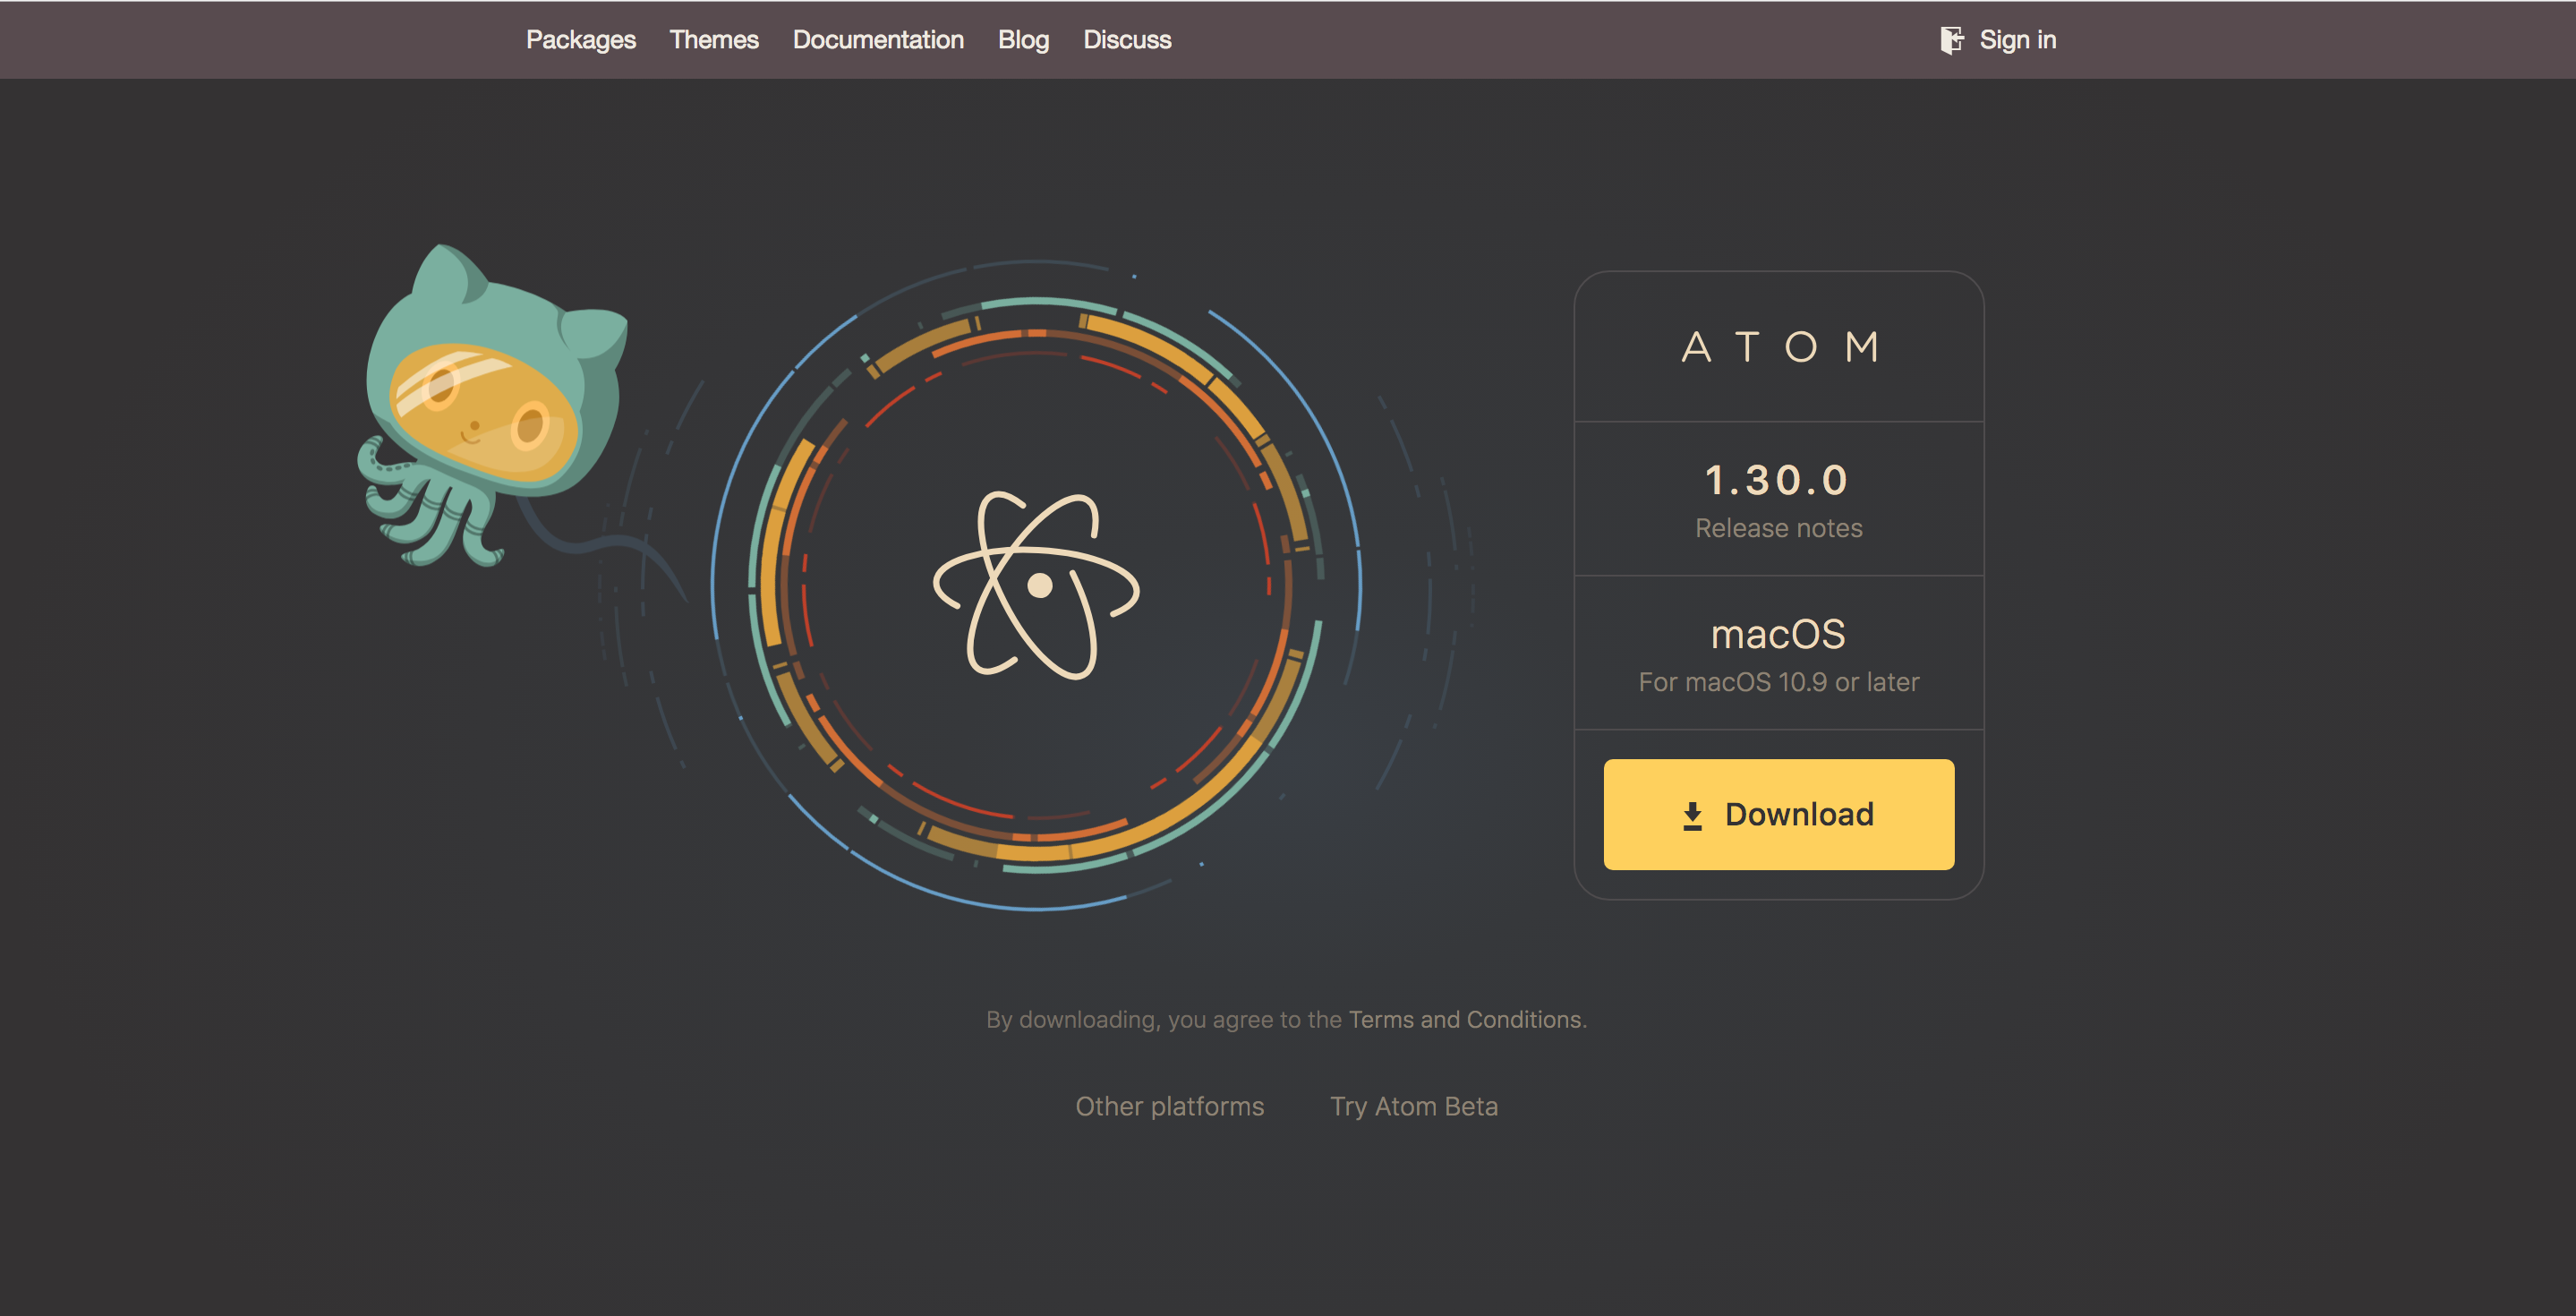
\includegraphics{atom-getting-started.png}
\item
  See the red \textbf{Download} button? Click it. Your computer should
  then download a .zip (Mac) or .exe (Win) file.~Some computers may
  automatically open and unpack the .zip file. If yours doesn't, then
  open the .zip file yourself. (If you don't know how to open .zip files
  on your computer, Google it.) Eventually, you should see the Atom
  icon.
\item
  If you're using a Mac, drag that icon to your \textbf{Applications}
  folder. If you're using Windows, Atom should automatically add an Atom
  shortcut to your \textbf{desktop} and your \textbf{Start menu}.~
\item
  Click the Atom icon to launch Atom!
\end{enumerate}

For more info/help, visit the
\href{http://flight-manual.atom.io/getting-started/sections/installing-atom/\#platform-mac}{Installing
Atom} section of the Atom documentation. Note that at the top of the
page you can choose your operating system (Windows or Mac).

\hypertarget{installing-packages}{%
\section{Installing packages}\label{installing-packages}}

Atom's a little different than Word. Word comes with a whole bunch of
features, most of which you'll never use. Atom comes with a few features
but allows you to quickly install many more. You install those features
via the \textbf{package manager}. Let's install most of the packages
we'll need this semester.

\begin{enumerate}
\def\labelenumi{\arabic{enumi}.}
\tightlist
\item
  Once you've launched Atom, you should see a screen with a Welcome
  Guide and other information. At the top of the screen, you should see
  a menu bar like you do with other applications (File, Edit, View,
  etc.). Open the Settings view by choosing \textbf{File =\textgreater{}
  Settings (Win)} or \textbf{Atom =\textgreater{} Preferences (Mac)}.
  Alternatively, if you want to be a baller, just hit \textbf{ctrl+comma
  (Win)} or \textbf{cmd+comma (Mac)}. You should see a screen like the
  one below.\\
  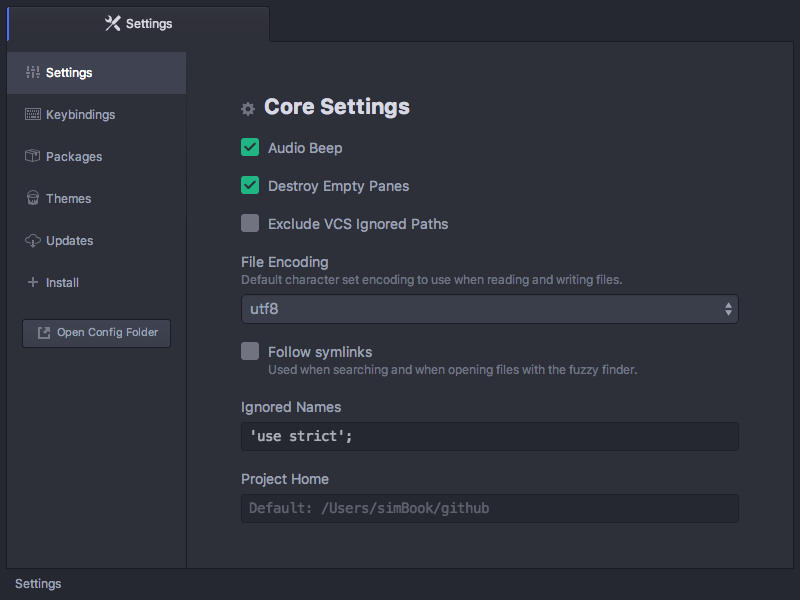
\includegraphics{atom-settings.png}
\item
  First, click the Editor tab, scroll down to \textbf{Soft Wrap}, and
  check the corresponding box.
\item
  Next, click the Themes tab. Here you can choose a dark background or a
  light background. If you prefer a dark background, do nothing. If you
  prefer a light background, choose One Light. Be sure to change both
  the UI Theme and the Syntax Theme.
\item
  Finally, click the Install tab. You should see a screen like the one
  below.\\
  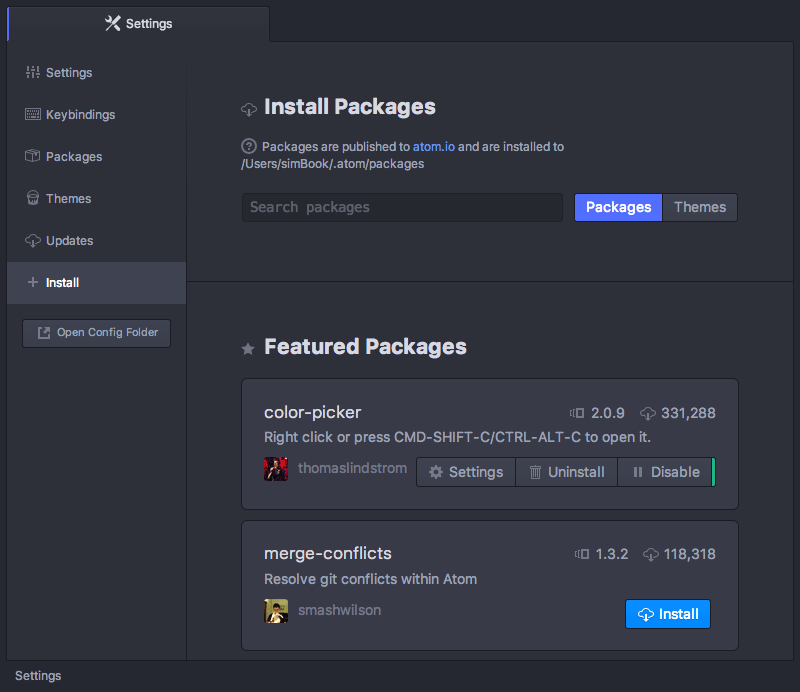
\includegraphics{packages-install.png}
\item
  In the Install Packages search bar, search for \textbf{atom-beautify}.
  When the package appears, click the \textbf{Install} button and wait
  for the installation to complete. Congrats--you've just installed a
  package!
\item
  Repeat step 5 for each of the packages below. Once you've installed
  the packages, you can view some of them in the Packages menu (in the
  same menu bar as File, Edit, View, etc.).

  \begin{itemize}
  \tightlist
  \item
    \textbf{atom-html-preview} -- allows you to view changes to your
    website from within Atom
  \item
    \textbf{emmet} -- allows you to write your code more quickly
  \item
    \textbf{linter} -- helps identify potential errors in your code.
    When you install this one, Atom may ask you to install
    ``dependencies.'' Allow each of these
  \item
    \textbf{markdown-writer} -- allows you to make pretty documents with
    no fuss (we'll use this one right away!)
  \item
    \textbf{tool-bar} -- with the next package, adds a toolbar with
    buttons for italics, etc.
  \item
    \textbf{tool-bar-markdown-writer} -- see directly above
  \item
    \textbf{pandoc-convert} -- converts Markdown files (see below) to
    Word docs, PDFs, or other formats
  \end{itemize}
\end{enumerate}

\hypertarget{optional-packages}{%
\section{Optional packages}\label{optional-packages}}

If you wish, you may also download these packages:

\begin{itemize}
\tightlist
\item
  \textbf{wordcount} -- adds a word count to the bottom of Atom's
  interface
\item
  \textbf{linter-write-good} -- tries to identify common writing issues
  (e.g., passive voice). Can be helpful, but when in doubt use your own
  judgment
\end{itemize}

\bibliography{book.bib,packages.bib}


\end{document}
